Onder de knop ``Magazijn'' kunt U de totale verbruikte producten per
pati\"ent of per afdeling vinden. Hieronder zullen we uitleggen hoe
dit in zijn werk gaat.\\
\\
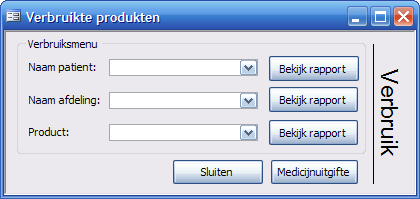
\includegraphics[scale=.7]{magazijn1}

\section{Verbruik per pati\"ent}\label{sec:verbruik_per_pati_ent} % (fold)

Voor het verbruik per pati\"ent selecteert U de patient door zijn
naam in het aangegeven veld te tikken of deze te selecteren uit de
lijst. Vervolgens klikt U op ``Bekijk rapport''. Een nieuw venster
verschijnt met de gevraagde gegevens.

% section verbruik_per_pati_ent (end)

\section{Verbruik per afdeling}\label{sec:verbruik_per_afdeling} % (fold)

Voor het verbruik per afdeling selecteert U de afdeling door die in
het aangegeven veld te tikken of deze te selecteren uit de lijst.
Vervolgens klikt U op ``Bekijk rapport''. Een nieuw venster
verschijnt met de gevraagde gegevens.

% section verbruik_per_afdeling (end)

\section{Verbruik per product}\label{sec:verbruik_per_product} % (fold)

Voor het verbruik per product selecteert U het product door die in
het aangegeven veld te tikken of deze te selecteren uit de lijst.
Vervolgens klikt U op ``Bekijk rapport''. Een nieuw venster
verschijnt met de gevraagde gegevens.

% section verbruik_per_product (end)

\section{Medicijnuitgifte}\label{sec:uitgifte van medicijnen} % (fold)

Om medicijnen uit te geven klikt U op de knop ``Uitgiftes''.
Onderstaand venster wordt geopend. Er worden namen van pati\"enten
weergegeven die \'e\'en of meerdere openstaande recepten hebben. De
openstaande recepten van een pati\"ent staan op datum gesorteerd.\\
\\
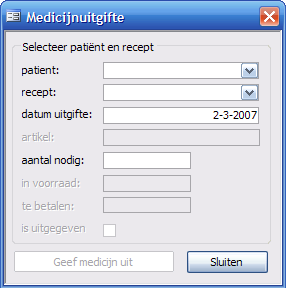
\includegraphics[scale=.7]{uitgifte1}

\subsection{Recept selecteren}\label{sec:recept selecteren} % (fold)

Selecteer de pati\"ent aan wie U een medicijn wilt uitgeven door de
naam in te typen of te selecteren uit de lijst. Selecteer vervolgens
de datum waarop het recept is voorgeschreven door de datum in te
typen of te selecteren uit de lijst. De naam van het medicijn waar
het recept voor is staat aangegeven naast de datum van uitgifte van
het recept.

\subsection{Datum van uitgifte}\label{sec:datum van uitgifte} % (fold)

De datum van uitgifte staat standaard ingesteld op de huidige datum,
maar deze kan aangepast worden, dit in verband met administratie van
eerder uitgegeven medicijnen die nog niet geregistreerd waren.

\subsection{Aantal eenheden}\label{sec:aantal eenheden} % (fold)

Het aantal eenheden medicijn dat moet worden uitgegeven wordt
automatisch berekend aan de hand van het recept. Mocht er toch een
aantal eenheden medicijn meer meegegeven moeten worden (bijvoorbeeld
omdat er per doosje meer eenheden verpakt zitten dan nodig voor de
pati\"ent) dan kan dit berekende aantal nog handmatig worden
aangepast.

\subsection{Uitschrijven}\label{sec:Uitschrijven} % (fold)

Om het medicijn uit te schrijven klikt U op de knop ``Geef medicijn uit''. Wanneer de gevraagde hoeveelheid medicijn in de
voorraad aanwezig is wordt het medicijn aan de klant meegegeven en
wordt de voorraad bijgewerkt. Het recept kan dan ook niet meer
worden uitgegeven en zal niet meer in de lijst met uitgeefbare
medicijnen te zien zijn. Als het medicijn niet voldoende op voorraad
is, kunt U het medicijn niet uitgeven en kan de pati\"ent het
medicijn op een later tijdstip komen ophalen. Het venster wordt
automatisch gesloten.

% section uitgifte (end)
